\subsection{Vermessung der Spektralinien}
\label{subsec:auswertung_spektrallinien}
\subsubsection{Reflexionsgitter}
Um die Wellenlänge der Emissionslinien zu bestimmen, wird ein Reflexionsgitter verwendet. Untersucht wird dabei die Lage der Interferenzmaxima des reflektierten Lichtes. Eine wichtige Größe, die das Gitter charakterisiert, ist dabei die Gitterkonstante $g$, die die Periode des Gitters angibt. Mit Hilfe von Abbildung \ref{Gangunterschied} lässt sich leicht der Gangunterschied $s$ zweier benachbarter Strahlen berechnen. Werden die Winkel in mathematisch positiver Richtung zum Lot gemessen erhält man
\begin{align*}
  s=g \cdot (\sin(\alpha)+\sin(\beta)).
\end{align*} 
Für Licht der Wellenlänge $\lambda$ gilt bei den Interferenzmaxima also (mit $n \in \mathbb{Z}$)
\begin{align}
  g \cdot (\sin(\alpha)+\sin(\beta)) = n\lambda.
  \label{equ:gitter}
\end{align}
\begin{figure}[h]
  \centering
  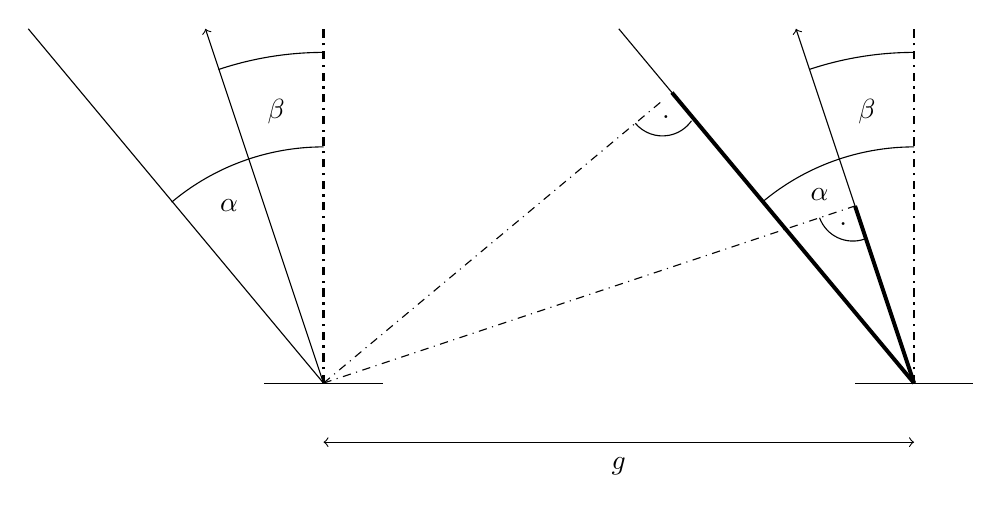
\begin{tikzpicture}[scale=1.5]
    \draw (0,0)--(1,0);
    \draw [thick, dash dot] (0.5,0)--(0.5,3);
    \draw (-2,3)--(0.5,0);
    \draw [->] (0.5,0)--(-0.5,3);
    \draw (0.5,2.8) arc (90:108.5:2.8);
    \draw (0.5,2) arc (90:130:2);
    \draw (0.1,2.3) node {$\beta$};
    \draw (-0.3,1.5) node {$\alpha$};
    \draw (5,0)--(6,0);
    \draw [thick, dash dot] (5.5,0)--(5.5,3);
    \draw (5.5-2.5,3)--(5.5-2.5*0.82,3*0.82);
    \draw [line width=0.5mm] (5.5-2.5*0.82,3*0.82)--(5.5,0);
    \draw [line width=0.5mm] (5.5,0)--(5.5-0.5,0.5*3);
    \draw [->] (5.5-0.5,0.5*3)--(4.5,3);
    \draw (5.5,2.8) arc (90:108.5:2.8);
    \draw (5.5,2) arc (90:130:2);
    \draw (5.1,2.3) node {$\beta$};
    \draw (4.7,1.6) node {$\alpha$};
    \draw [dash dot](0.5,0)--(0.5+2.4*6/5,2.4);
    \draw [dash dot](0.5,0)--(0.5+1.5*3,1.5);
    \draw [<->] (0.5,-0.5)--(5.5,-0.5);
    \draw (3,-0.7) node {$g$};
    \draw (0.5+2.2*6/5,2.2) arc (220:325:0.3);
    \draw (3.4,2.25) node {$.$};
    \draw (0.5+1.4*3,1.4) arc (200:290:0.3);
    \draw (4.9,1.35) node {$.$};
  \end{tikzpicture}
  \caption{Gangunterschied (fett eingezeichnet) für benachbarte Strahlen}
  \label{Gangunterschied}
\end{figure}

Im Experiment kann man allerdings die Winkel $\alpha$ und $\beta$ nicht direkt messen, sondern man misst die Winkel $\omega\ind{G}$ und $\omega\ind{B}$ (siehe Abb. \ref{aufbau2}). Daraus ergibt sich:
\begin{align}
\alpha = \omega\ind{G}, \beta = \omega\ind{G}+\omega\ind{B}-180^\circ.
\label{equ:angle}
\end{align}
Während des gesamten Versuches war $\omega\ind{B}=150^\circ \pm 0,5^\circ$.

\subsubsection{Bestimmung der Gitterkonstanten}
\begin{figure}[h]
  \centering
  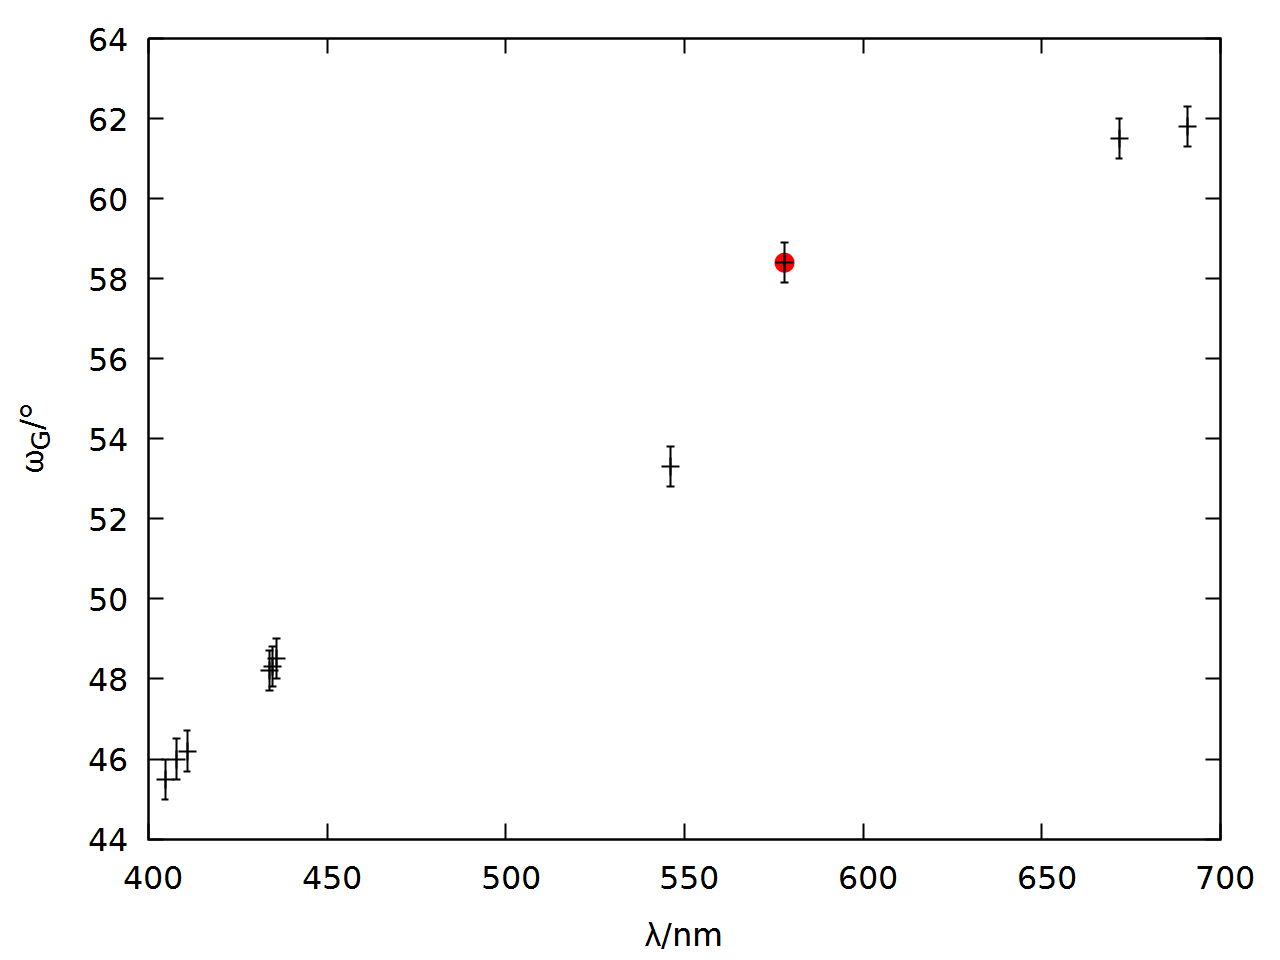
\includegraphics[width=0.75\linewidth]{data/Balmer/out_hg_raw.png}
  \caption{Gemessene Winkel $\omega\ind{G}$ der Spektralinien der Hg-Lampe}
  \label{fig:hg_raw}
\end{figure}

Da man die beiden gelben Linien nicht unterscheiden konnte, haben wir für die Wellenlänge der gelben Linie (roter Punkt, siehe Abb. \ref{fig:hg_raw}) den Mittelwert beider Linien angesetzt: $\lambda = \si{(578,013 \pm 1,053) \nano \metre}$. Nach Gl. \ref{equ:angle} werden $\alpha$ und $\beta$ berechnet. In Abb. \ref{fig:hg} ist $\lambda$ über $\sin{\alpha} + \sin{\beta}$ aufgetragen \footnote{$\Delta \sin{\alpha} = |\cos{\alpha} \cdot \Delta \alpha|$, $\Delta beta$ analog}. Zusätzlich ist in das Diagramm ein linearer Fit $y = a\cdot x + b$ an diese Daten eingezeichnet.
\begin{figure}[h]
  \centering
  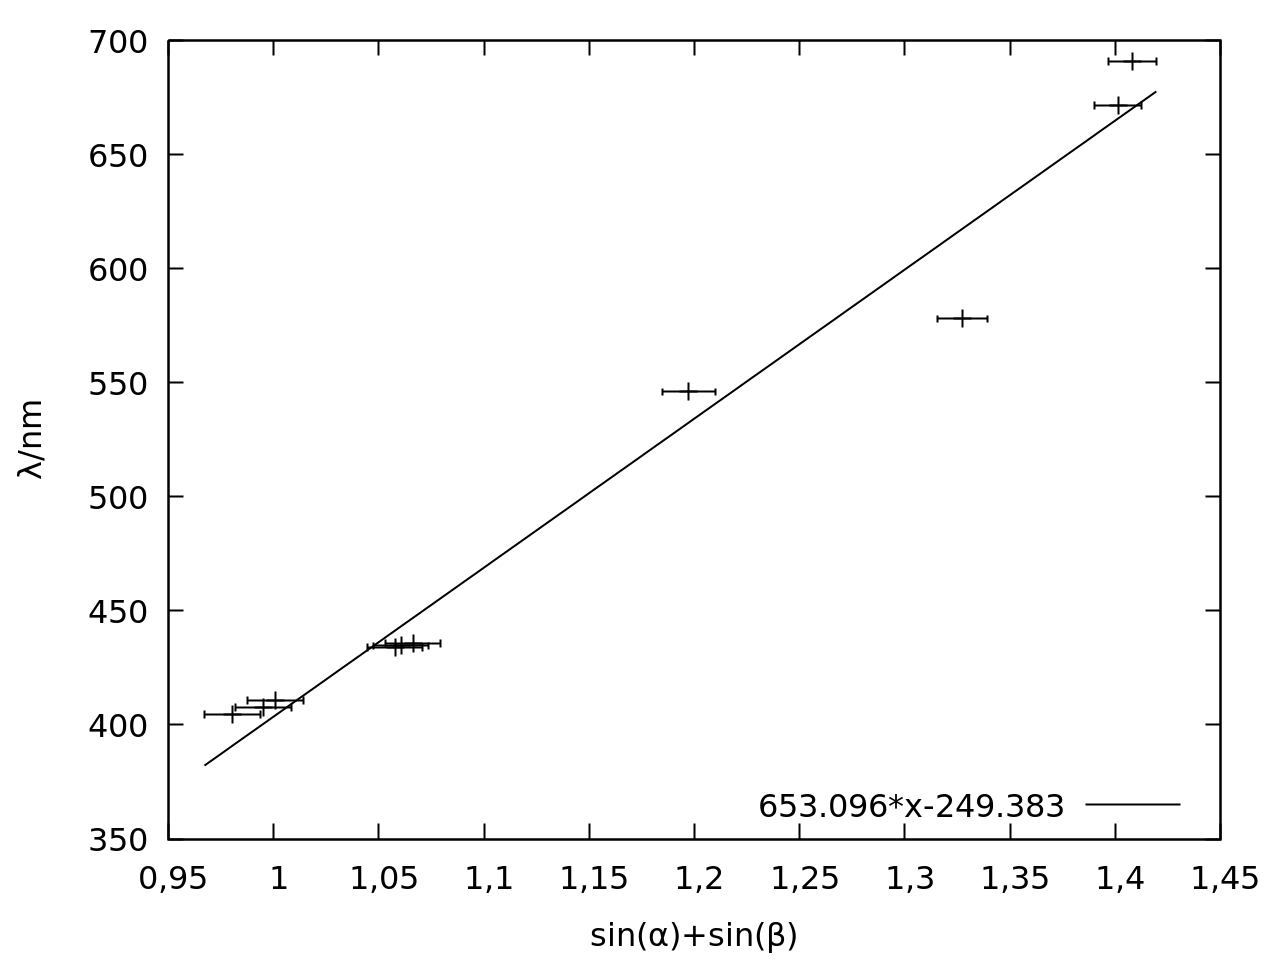
\includegraphics[width=0.75\linewidth]{data/Balmer/out_hg.png}
  \caption{Bestimmung der Gitterkonstante}
  \label{fig:hg}
\end{figure}

Der Fit ergibt $a = \si{(653 \pm 36) \nano\metre}, b = \si{(-249 \pm 43) \nano\metre}$. Die Gitterkonstante beträgt also $g = a = \si{(653 \pm 36) \nano\metre}$. Nach Gl. \ref{equ:gitter} sollte $b \approx 0$ sein. Dies könnte aufgrund eines kleinen systematischen Fehlers auftreten (z.B. ein kleiner Offset bei der Winkelmessung). Extrapoliert man die Funktion bis $x = 0$, so liegt $\lambda = 0$ im Fehlerbereich. Führt man einen Fit ohne Achsenabschnitt $y = a\cdot x$ durch, so ergibt sich: $\si{(444 \pm 11) \nano\metre}$. Allerdings passt sich ein Fit mit Achsenabschnitt besser den Daten an, weswegen wir  entschieden haben, mit der Relation
\begin{align}
\lambda = g (\sin{\alpha} + \sin{\beta}) + b
\label{equ:gitter_neu}
\end{align}
weiterzuarbeiten.

\subsubsection{Untersuchung der Balmerlinien mit Okular}

\begin{table}
\centering
\caption{Messung mit dem Okular}
\begin{tabular}{c>{$}c<{$}>{$}c<{$}}
\toprule
Linie & \omega\ind{G}/^\circ & d/\si{\milli \metre}\\
\midrule
H$_\alpha$ & 60,5 \pm 0,5 &0,1\pm 0,05\\
H$_\beta$ & 53	\pm 0,5 &0,3\pm 0,05\\ 
H$_\gamma$ & 48,5 \pm 0,5\\
H$_\delta$ & 48\pm 0,5\\
H$_\epsilon$ & 46\pm 0,5\\
\bottomrule
\end{tabular}
\label{tab:okular}
\end{table}

In Tab. \ref{tab:okular} sind die gemessenen Winkel und die Aufspaltung der einzelnen Linien eingetragen. Die Aufspaltung konnte nur für die H$_\alpha$- und H$_\beta$-Linie bestimmt werden. Die Wellenlängen der Linien wurden über Gl. \ref{equ:angle} und Gl. \ref{equ:gitter_neu} berechnet. Um die Isotopieaufspaltung $\delta \lambda$ zu berechnen, linearisiert man Gl. \ref{equ:gitter_neu}: $\delta \lambda = g\cos{\beta} \delta\beta$. $\delta \beta$ ergibt sich aufgrund des nahezu parallelen Lichtes durch: $\delta\beta = \arctan{\frac{d}{f}} \overset{d \ll f}{=} \frac{d}{f}$, wobei $f$ die Brennweite des Objektives ist. Da wir keine Angabe über den Fehler von $f$ haben, haben wir den Fehler auf \si{10\milli \metre} geschätzt: $f = \si{(300\pm 10)\milli \metre}$.\\

In \ref{tab:okular_res} sind die berechneten Wellenlängen, die Isotopieaufspaltung sowie die theoretischen Werte angeben. Die wirklichen Wellenlängen liegen alle im Fehlerbereich der berechneten Werte.\\

\begin{table}
\centering
\caption{Ergebnisse der Messung mit dem Okular}
\begin{tabular}{c>{$}c<{$}>{$}c<{$}>{$}c<{$}}
\toprule
Linie & \lambda/\si{\nano\metre} & \lambda\upd{theo}/\si{\nano\metre} & \delta\lambda/\si{\nano \metre}\\
\midrule
H$_\alpha$ & 651\pm 56 & 656,278 & 0,19\pm 0,09\\
H$_\beta$ & 527 \pm	53 & 486,132 & 0,6\pm 0,1\\ 
H$_\gamma$ & 447 \pm 50 & 434,045\\
H$_\delta$ & 438 \pm 50 & 410,1735\\
H$_\epsilon$ & 400 \pm 49 & 397,0074\\
\bottomrule
\end{tabular}
\label{tab:okular_res}
\end{table}

Aus den Daten wird die Rydbergkonstante $R_\infty$ nach Gl. \ref{equ:rydberg} bestimmt, indem man $\frac{1}{\lambda}$ über $\frac{1}{2^2}-\frac{1}{n^2}$ ($n = 3,4,5,6,7$) aufträgt und einen linearen Fit $y = R \cdot x$ durchführt. (siehe Abb. \ref{fig:rydberg}).

\begin{figure}[h]
  \centering
  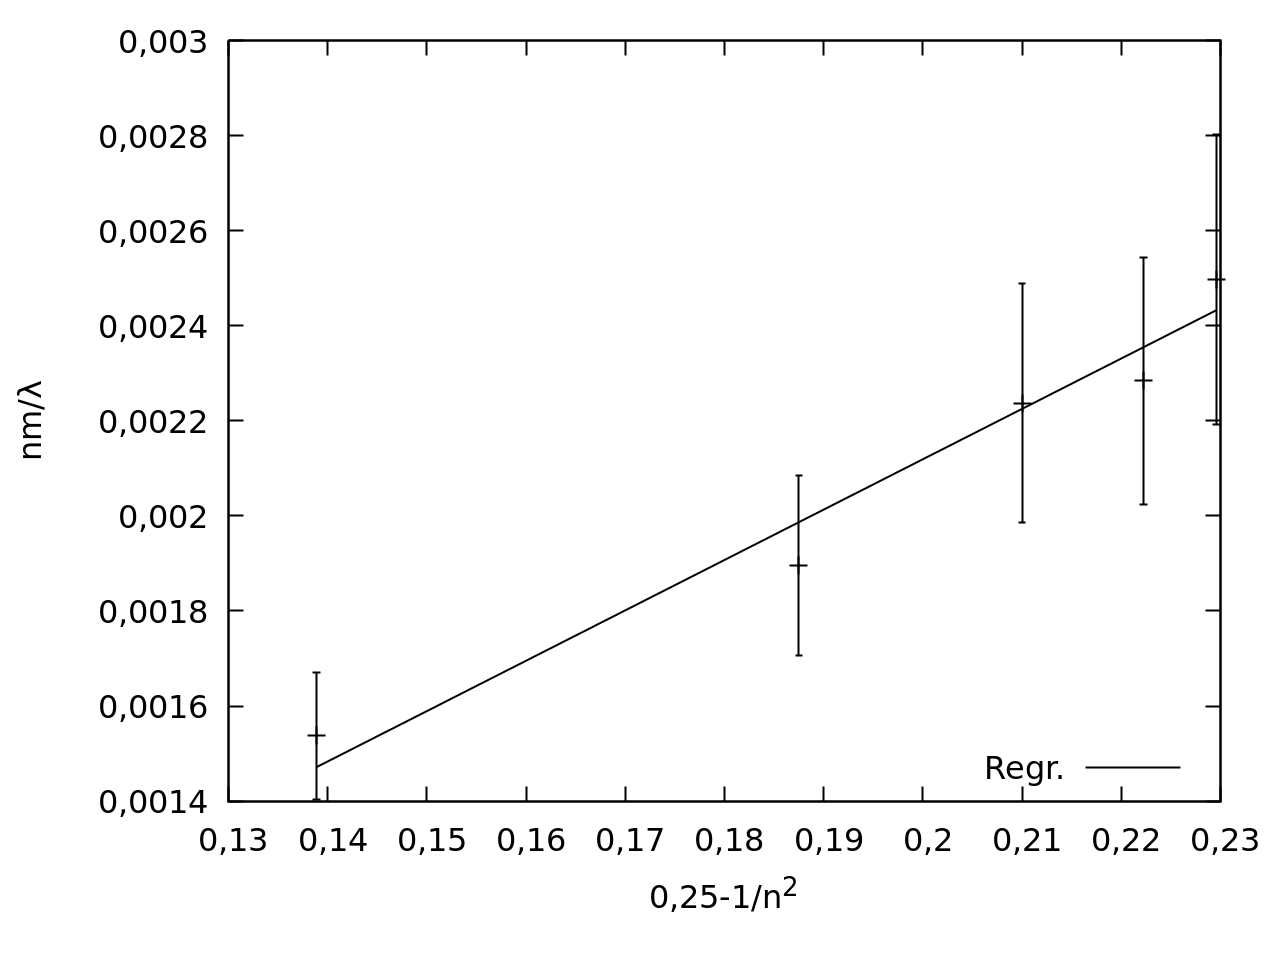
\includegraphics[width=0.75\linewidth]{data/Balmer/out_rydberg.png}
  \caption{Bestimmung der Rydbergkonstanten}
  \label{fig:ryberg}
\end{figure}

Der Fit ergibt: $R = (10,6 \pm 0,2)\cdot 10^6\frac{1}{\si{\metre}}$. $R_\infty$ ergibt sich nun durch $R_\infty = (1+\frac{m\ind{e}}{m\ind{p}}) R = (10,6 \pm 0,2)\cdot 10^6\frac{1}{\si{\metre}}$ (Massen der Teilchen aus \cite{wiki_konst}). Der Literaturwert \cite{wiki_konst} ist $10,97 \cdot 10^6\frac{1}{\si{\metre}}$. Unser Wert liegt also in der gleichen Größenordnung, wie der wahre Wert. Allerdings liegt dieser knapp nicht im Fehlerintervall. Für das Wirkungsquantum $h = \sqrt[3]{\cfrac{m\ind{e}\mathrm{e}^4}{8\epsilon_0^2R_\infty c}}$ ergibt sich (Konstanten \cite{wiki_konst}): $h = (6,8 \pm 0,1) \cdot 10^{-34} \si{\joule \second}$. Wie bei der Rydbergkonstante liegt der Literaturwert: $h = 6,63 \cdot 10^{-34} \si{\joule \second}$ recht nah an dem gemessenem Wert, allerdings knapp nicht im Fehlerintervall.

\subsubsection{Untersuchung der Balmerlinien mit CCD-Kamera}
Die Programm berechnet eigenständig aus der Pixelkoordinate den dazugehörigen Winkel $\delta  \beta = \gamma$. 

\begin{figure}[h]
  \centering
  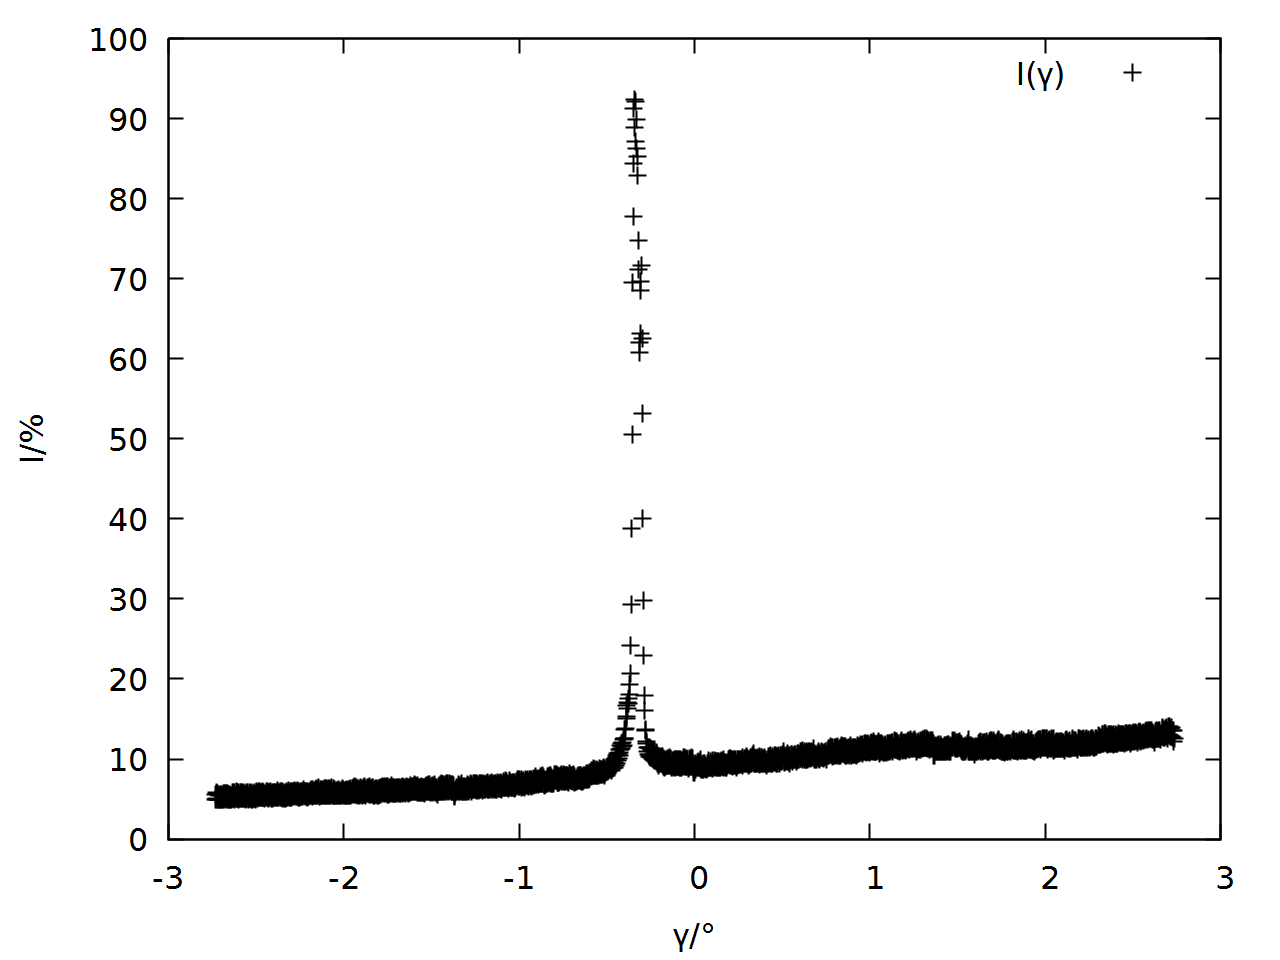
\includegraphics[width=0.75\linewidth]{data/Balmer/out_red_raw.png}
  \caption{Intensitätsverteilung der H$_\alpha$-Linie}
  \label{fig:red_raw}
\end{figure}
\begin{figure}[h]
  \centering
  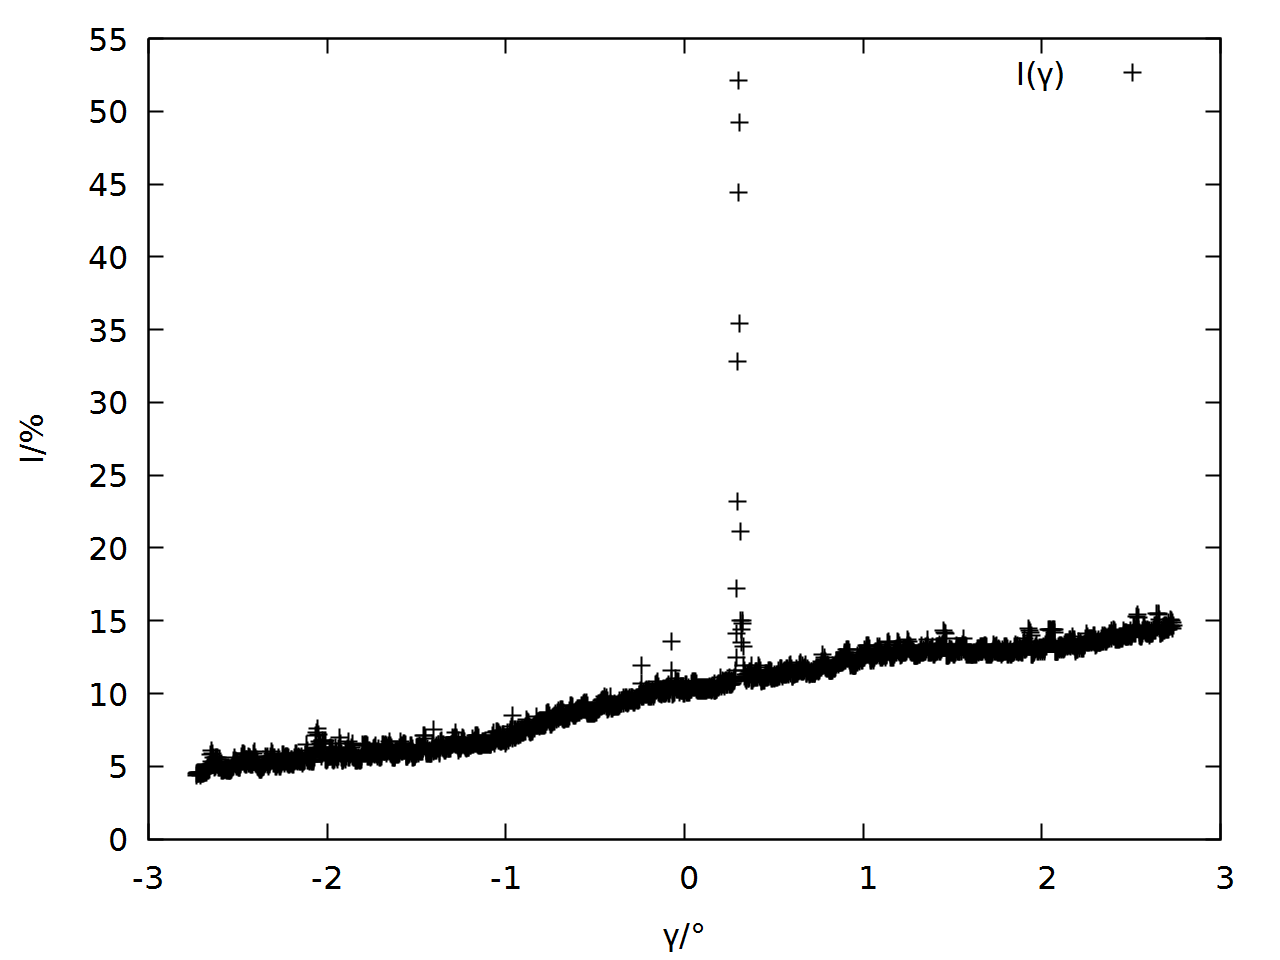
\includegraphics[width=0.75\linewidth]{data/Balmer/out_lightblue_raw.png}
  \caption{Intensitätsverteilung der H$_\beta$-Linie}
  \label{fig:lightblue_raw}
\end{figure}
\begin{figure}[h]
  \centering
  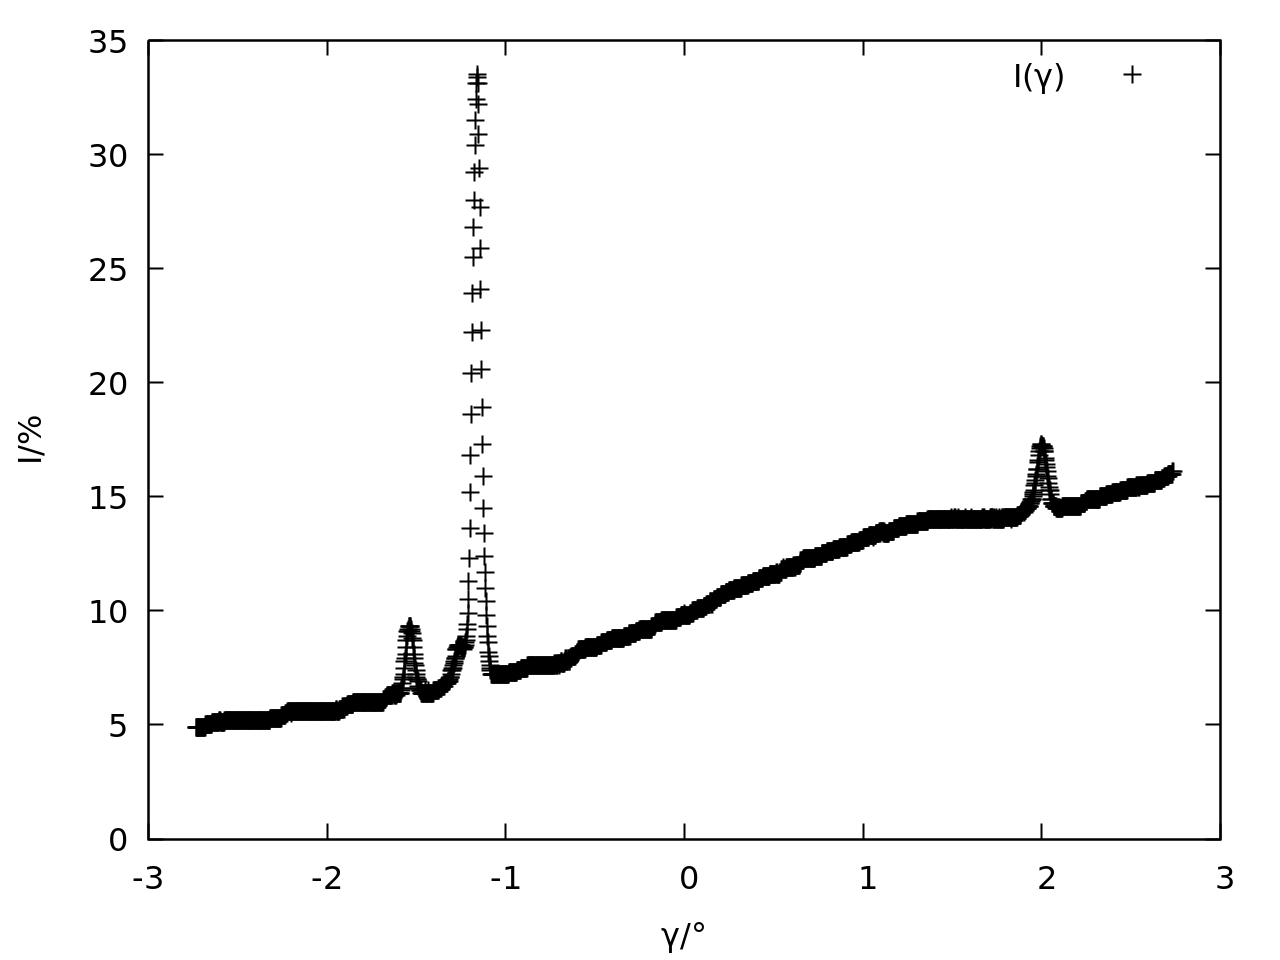
\includegraphics[width=0.75\linewidth]{data/Balmer/out_blue_raw.png}
  \caption{Intensitätsverteilung der (v.l.n.r.) H$_\gamma$-,H$_\delta$- und H$_\epsilon$-Linie}
  \label{fig:blue_raw}
\end{figure}

In den Abbildungen \ref{fig:red_raw}-\ref{fig:blue_raw} sind die von der Kamera gemittelten Werte aufgetragen. Da wir keine Angaben zu den Fehlern der Kamera haben (sowohl für $\gamma$, als auch für die Intensität $I$), sind keine Fehler in den Diagrammen eingezeichnet. Für das weitere Vorgehen ist dies nicht relevant, da, wenn der Fehler für alle Werte gleich ist, das Ergebnis des Fitalgorithmus nicht beeinflusst wird. In Abb. \ref{fig:blue_raw} sind die drei blauen Balmer-Linien zu sehen. Vergleicht man die Abstände der Linien mit den Messungen des vorherigen Teils, so kann man erkennen, dass größere $\gamma$ kleineren Wellenlängen entsprechen.\\

Nun wird um jede Linie ein möglichst kleiner Ausschnitt genommen (siehe Abb. \ref{fig:red} - \ref{fig:blue2}). Kann man in diesem Ausschnitt 2 getrennte Linien erkennen (H$_\alpha$, H$_\beta$, H$_\delta$), wird an ihn die Summe zweier Gaussfunktionen angefittet:
\begin{align*}
I(\gamma) = a_1\exp{-\frac{(\gamma-b_1)^2}{2s_1^2}} + a_2\exp{-\frac{(\gamma-b_2)^2}{2s_2^2}} + d
\end{align*}
Leider war die Intensität der H$_\gamma$- und H$_\epsilon$-Linie nicht groß genug, um zwei Linien erkennen zu können. Deswegen wird nur eine Gaussfunktion an den Ausschnitt gefittet:
\begin{align*}
I(\gamma) = a_1\exp{-\frac{(\gamma-b_1)^2}{2s_1^2}} + d
\end{align*}
Das d haben wir aufgrund eines nicht vernachlässigbaren Untergrundes hinzugefügt. Die Ergebnisse der Fits sind in Tab. \ref{tab:ccd_fit} dargestellt.

\begin{figure}[h]
  \centering
  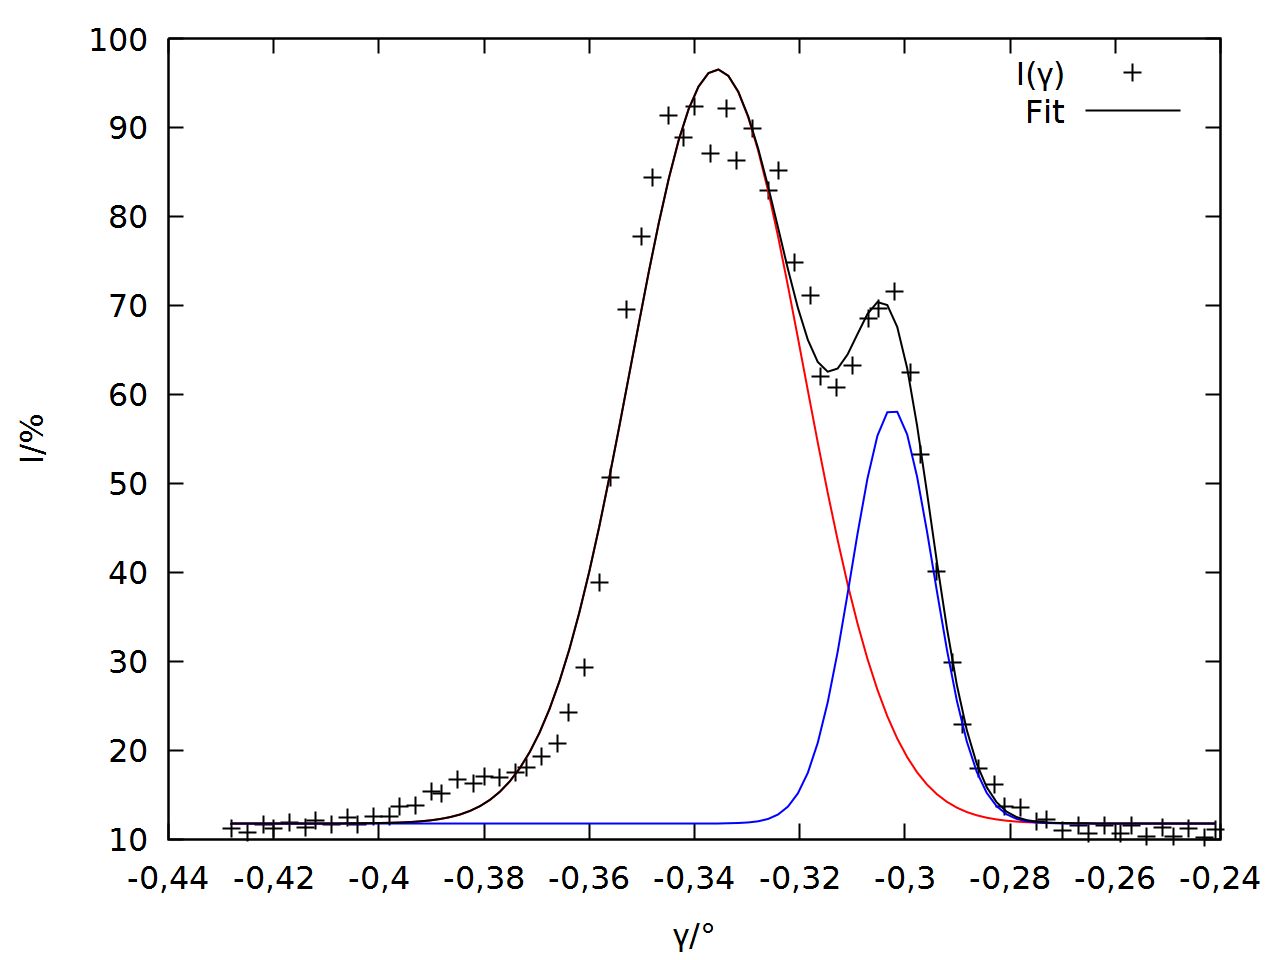
\includegraphics[width=0.75\linewidth]{data/Balmer/out_red.png}
  \caption{Fit an die H$_\alpha$-Linie}
  \label{fig:red}
\end{figure}
\begin{figure}[h]
  \centering
  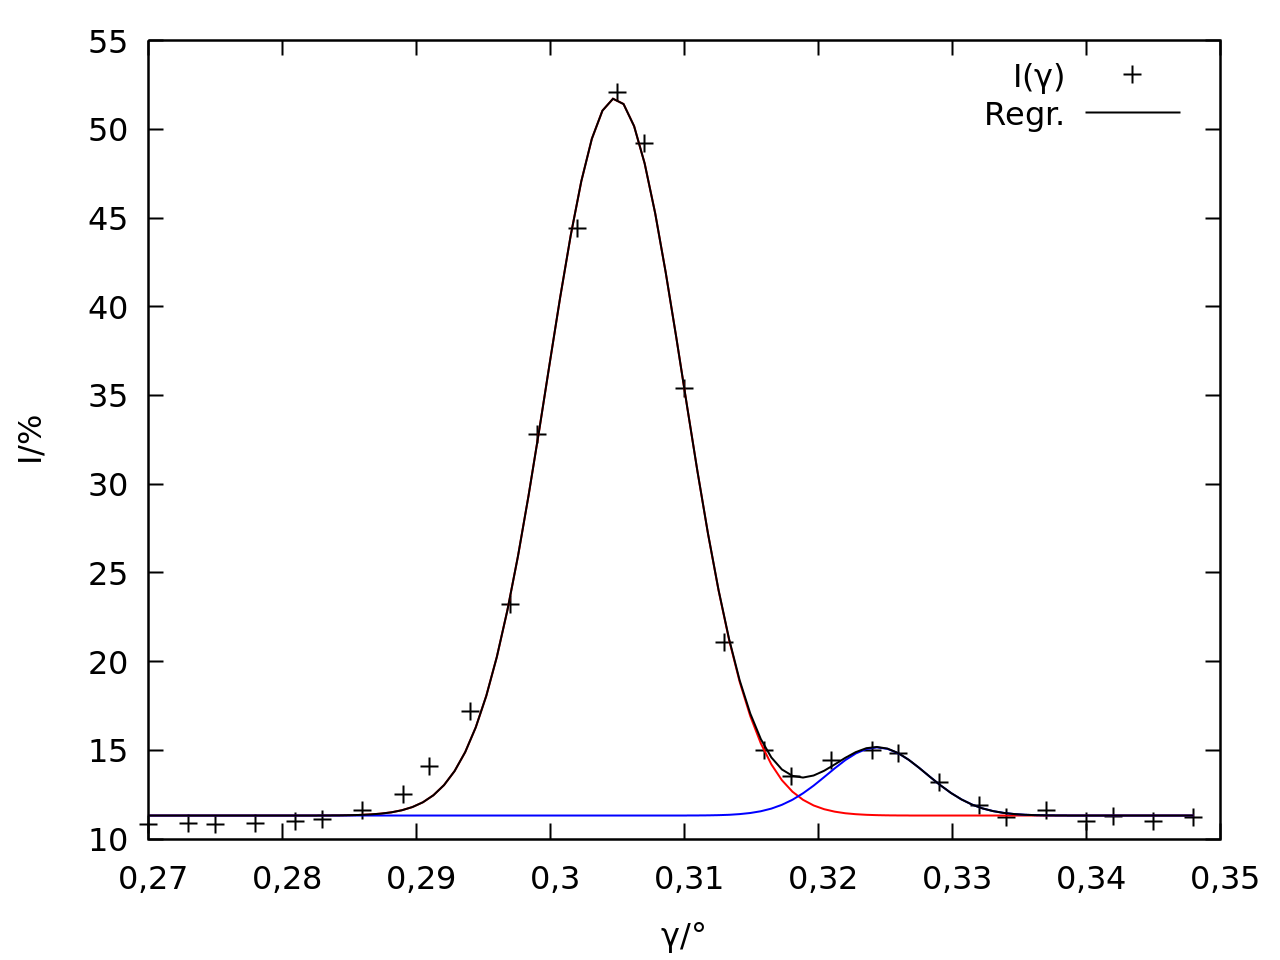
\includegraphics[width=0.75\linewidth]{data/Balmer/out_lightblue.png}
  \caption{Fit an die H$_\beta$-Linie}
  \label{fig:lightblu}
\end{figure}
\begin{figure}[h]
  \centering
  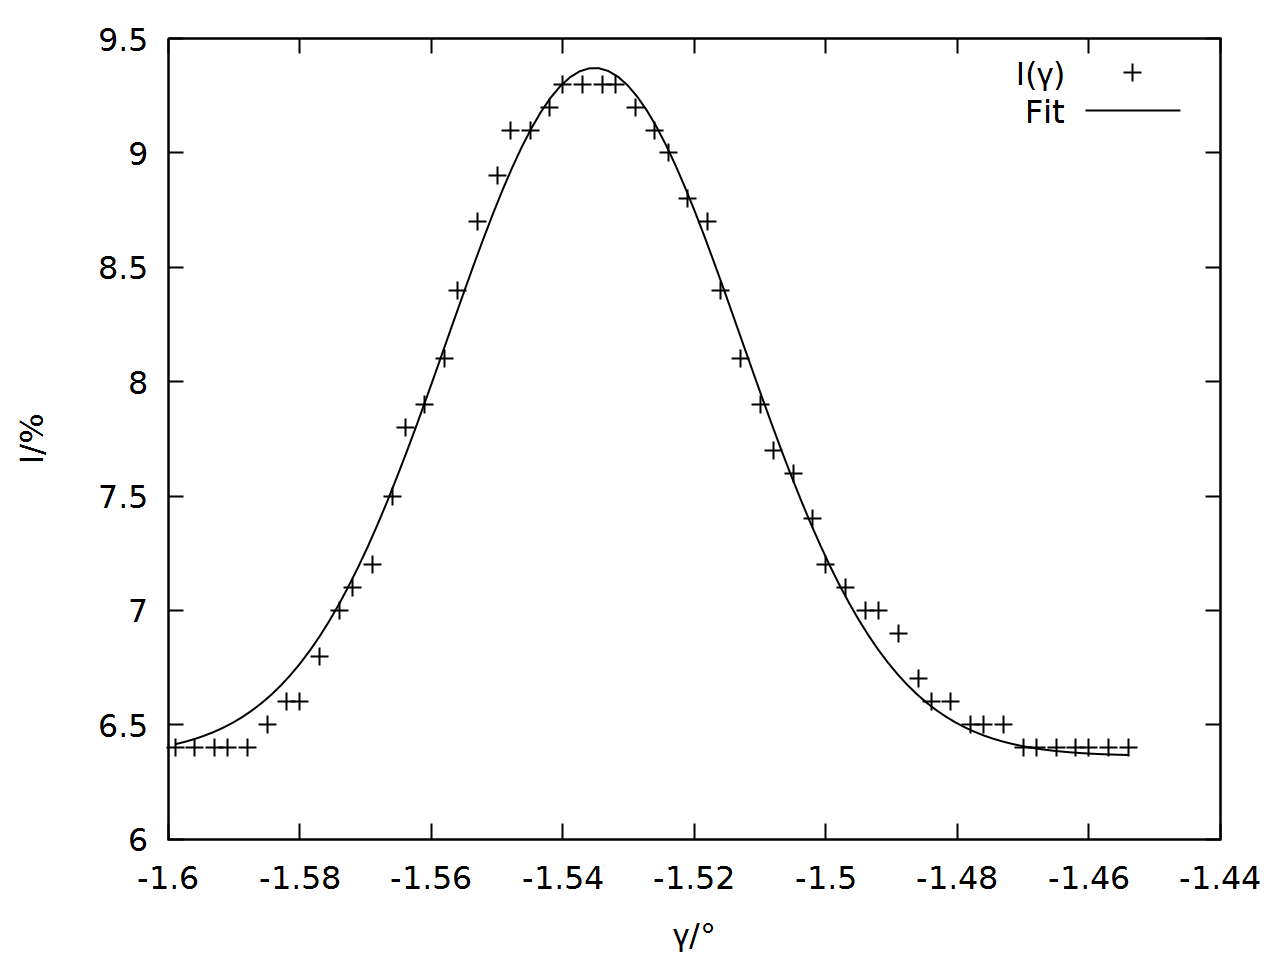
\includegraphics[width=0.75\linewidth]{data/Balmer/out_blue0.png}
  \caption{Fit an die H$_\gamma$-Linie}
  \label{fig:blue0}
\end{figure}
\begin{figure}[h]
  \centering
  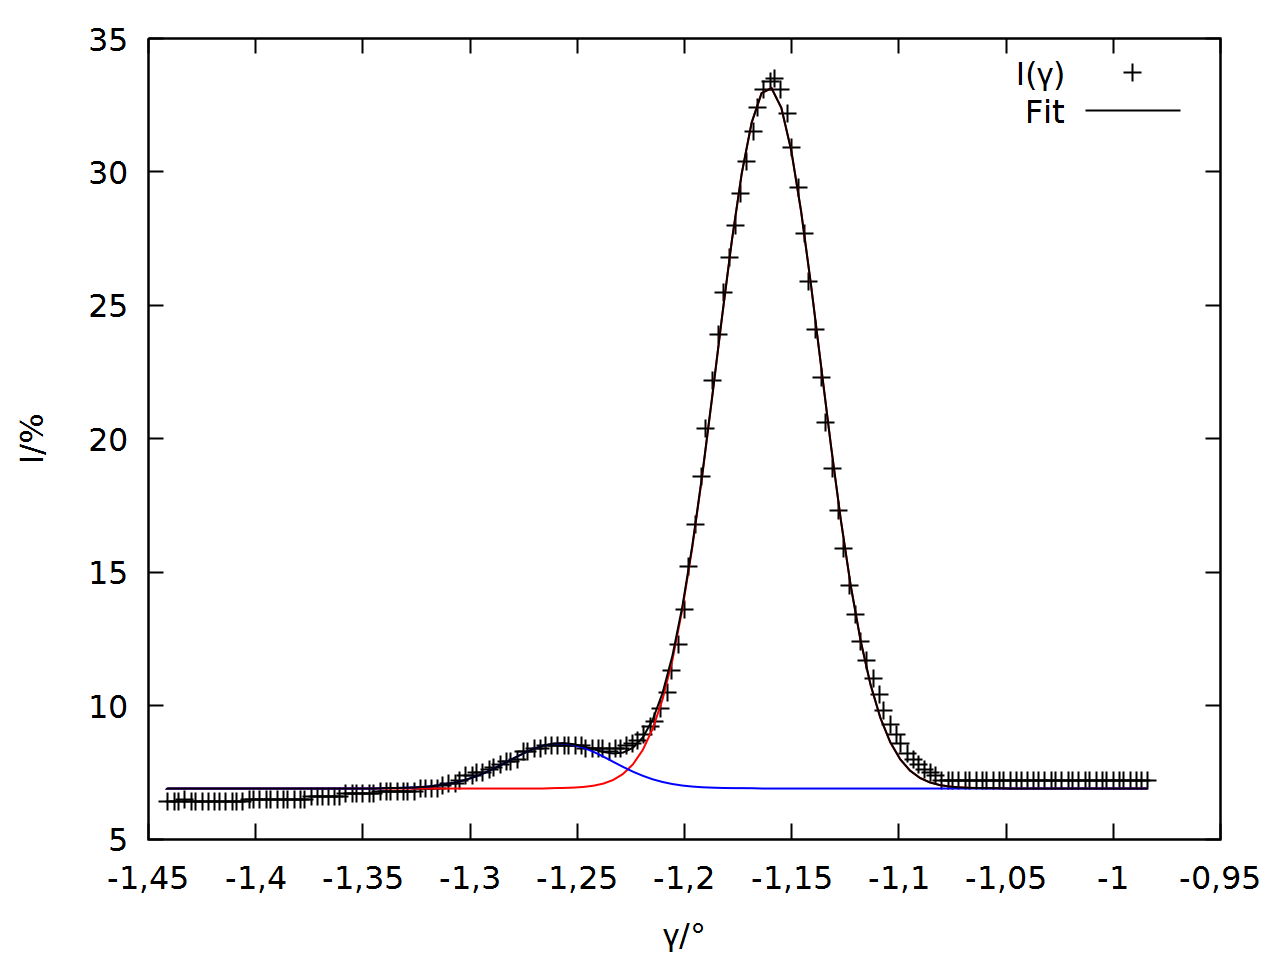
\includegraphics[width=0.75\linewidth]{data/Balmer/out_blue1.png}
  \caption{Fit an die H$_\delta$-Linie}
  \label{fig:blue1}
\end{figure}
\begin{figure}[h]
  \centering
  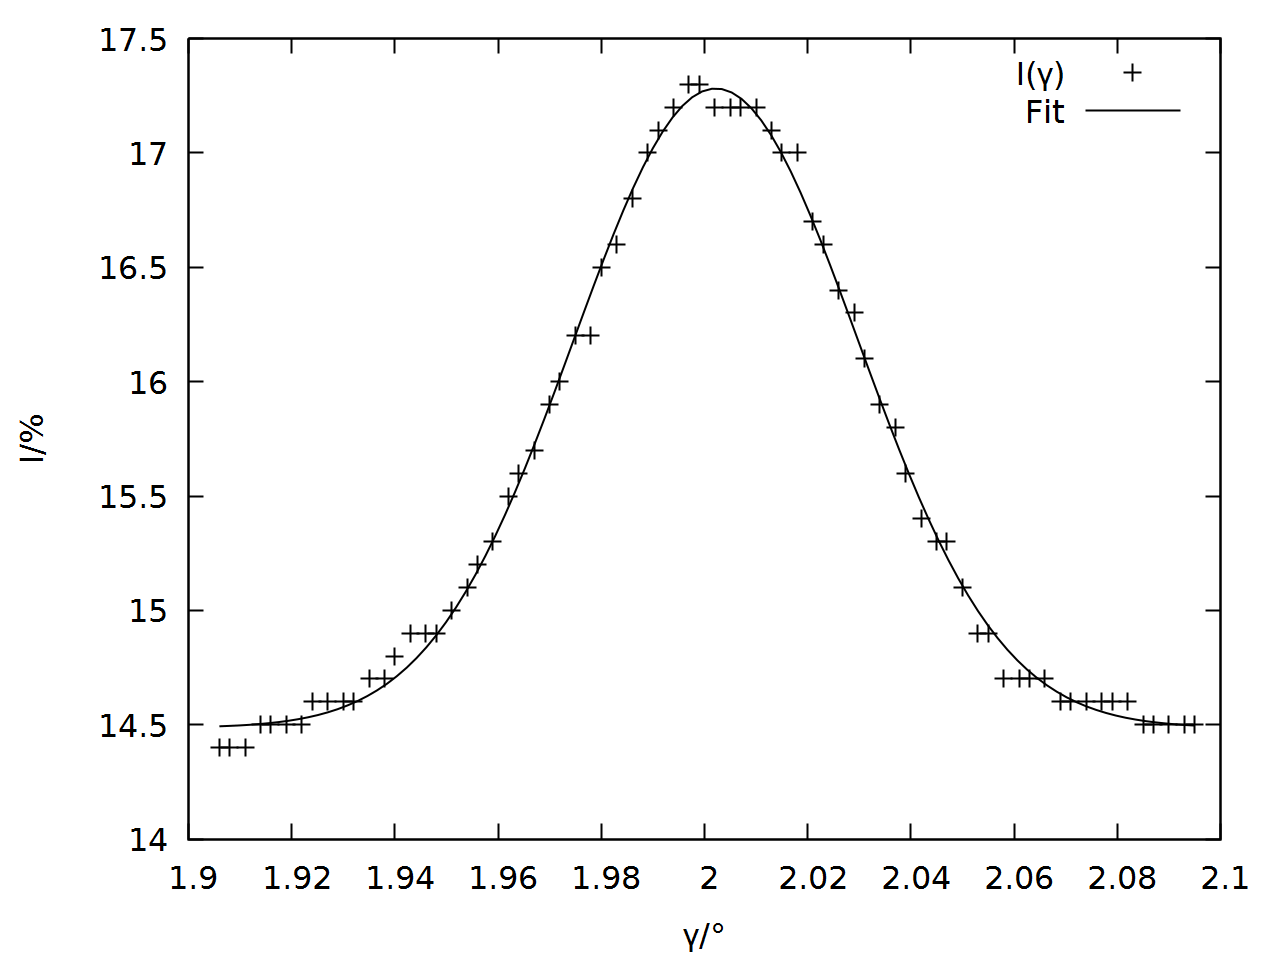
\includegraphics[width=0.75\linewidth]{data/Balmer/out_blue2.png}
  \caption{Fit an die H$_\epsilon$-Linie}
  \label{fig:blue2}
\end{figure}

\begin{table}[h]
%\centering
\caption{Ergebnisse der Fits an die Linien}
\begin{tabular}{>{$}c<{$}>{$}c<{$}>{$}c<{$}>{$}c<{$}>{$}c<{$}>{$}c<{$}}
\toprule
& H_\alpha & H_\beta & H_\gamma & H_\delta & H_\epsilon\\
\midrule
a_1/\% & 85 \pm 1 	& 40,4 \pm 0,5 	& 3,01 \pm 0,03	& 26,3 \pm 0,1 	& 2,79\pm 0,02\\
a_2/\% & 47 \pm 2 	& 3,8\pm 0,6 	& 	& 1,7 \pm 0,1 \\ 		
b_1/^\circ & -0,3357 \pm 5\cdot 10^{-4} & 0,30481\pm 8\cdot 10^{-5} & -1,5352\pm 2\cdot 10^{-4} & -1,1607 \pm 1\cdot 10^{-4} & 2,0022 \pm 2\cdot 10^{-4}\\
b_2/^\circ & -0,3024 \pm 5 \cdot 10^{-4}	& 0,3244\pm 7\cdot 10^{-4} 	& 	& -1,258 \pm 1\cdot 10^{-3} 	&\\
s_1/^\circ & 0,0164 \pm 5\cdot 10^{-4} & 0,00508\pm 8\cdot 10^{-5} 	& 0,0223\pm 3\cdot 10^{-4} & 0,0243 \pm 1\cdot 10^{-4} 	&  0,0276\pm 3\cdot 10^{-4}\\
s_2/^\circ & 0,0078 \pm 5\cdot 10^{-4} 	& 0,0037\pm 7\cdot 10^{-4} & & 0,024\pm 2\cdot 10^{-3}	\\
d/\% & 11,7 \pm 0,6	& 11,3 \pm 0,2	& 6,36\pm 0,02 & 6,91  \pm 0,04 & 14,49\pm 0,01\\
\midrule
\delta\beta/^\circ & (5,8\pm 0,1)\cdot 10^{-4}  & (3,4\pm 0,1) \cdot 10^{-4}& & (-17,0\pm 0,3)\cdot 10^{-4}\\
\delta\lambda/\si{\nano\metre} & 0,33\pm 0,02 & 0,21\pm	0,01& & -1.05\pm 0,06\\
\bottomrule
\end{tabular}
\label{tab:ccd_fit}
\end{table}

Aus den Parametern kann man nun $\delta \beta = b_2-b_1$ berechnen ($b_1$ ist immer der höhere Peak). Der kleinere Peak entspricht der Deuteriumslinie, da das Gas weniger Deuterium enthält. Bei der H$_\alpha$- und H$_\beta$-Linie ist dieser rechts vom größeren Peak. Das ist auch zu erwarten, da die Linien des Deuteriums kleinere Wellenlängen haben, als die vom Wasserstoff. Nur bei der H$_\delta$-Linie liegt der kleinere Peak links vom größeren Peak (Deswegen sind $\delta\beta$ und $\delta \lambda$ negativ). Nach der Theorie sollten außerdem die Abstände der Linien mit abnehmender Wellenlänge kleiner werden. Der Abstand der Linie betrug aber etwa das dreifache des Abstandes der H$_\alpha$-Linie. Vermutlich handelt es sich also bei dem zweitem Gauss-Peak nicht um die Deuteriumslinie. Es könnte z.B. eine andere Spektrallinie im Hintergrund sein, oder, da der Peak sehr schwach ist, einfach Teil des Untergrundes. Wir betrachten deswegen diesen Wert nicht weiter.\\

\begin{table}
\centering
\caption{Berechnete Isotopieaufspaltungen mit Okular, mit CCD und der theoretische Wert}
\begin{tabular}{c>{$}c<{$}>{$}c<{$}>{$}c<{$}}
\toprule
Linie & \delta\lambda\upd{oku}/\si{\nano \metre} & \delta\lambda\upd{ccd}/\si{\nano \metre} & \delta\lambda\upd{theo}/\si{\nano \metre}\\
\midrule
H$_\alpha$ & 0,19\pm 0,09 & 0,33\pm 0,02 & 0,178\\
H$_\beta$ & (0,6\pm 0,1) & 0,21\pm 0,01 & 0,132\\
H$_\delta$ & 			 & (-1.05\pm 0,06) & 0,111\\
\bottomrule
\end{tabular}
\label{tab:ccd_res}
\end{table}

Stellt man alle Werte gegenüber, so kann man erkennen (siehe Tab. \ref{tab:ccd_res}), dass nur die Aufspaltung der H$_\alpha$-Linie bei der Messung mit dem Okular einen Wert liefert, der in der Nähe des theoretischen Wertes ist. Beide Werte der CCD-Messung liegen zwar in der gleichen Größenordnung, sind aber etwa doppelt so groß. Eine mögliche Fehlerquelle hierfür könnte die Berechnung von $\gamma$ sein. Diese basiert darauf, dass der Abstand zwischen Objektiv und Kamera der Brennweite entspricht. Geht man von einem Fehler von $1\si{\centi\metre}$ aus, so ergibt sich allerdings nur ein relativer Fehler von $\frac{\Delta f}{f} = \frac{\si{1\centi\metre}}{\si{30 \centi\metre}} = 3.3\%$. Somit muss es noch weitere größere Fehler geben.

